\subsection*{Problema 10}
\textbf{Enunciado:} Calcular la integral:
\begin{equation*}
\int \sqrt{x^2 + x + 1} \, dx
\end{equation*}

\textbf{Solución:} Para resolver la integral, comenzamos completando el cuadrado en el radicando:
\begin{align*}
x^2 + x + 1 &= \left(x^2 + x + \dfrac{1}{4}\right) + 1 - \dfrac{1}{4} \\
&= \left(x + \dfrac{1}{2}\right)^2 + \dfrac{3}{4}
\end{align*}

Sustituyendo esta expresión en la integral, obtenemos:
\begin{equation*}
\int \sqrt{\left(x + \dfrac{1}{2}\right)^2 + \dfrac{3}{4}} \, dx
\end{equation*}

Utilizamos la sustitución trigonométrica. 
Sea $x + \dfrac{1}{2} = \dfrac{\sqrt{3}}{2} \tan(\theta)$, de donde:
\begin{align*}
dx &= \dfrac{\sqrt{3}}{2} \sec^2(\theta) \, d\theta
\end{align*}

Además, la raíz cuadrada se transforma en:
\begin{align*}
\sqrt{\left(x + \dfrac{1}{2}\right)^2 + \dfrac{3}{4}} &= \sqrt{\dfrac{3}{4}\tan^2(\theta) + \dfrac{3}{4}} \\
&= \dfrac{\sqrt{3}}{2} \sec(\theta)
\end{align*}

Sustituyendo en la integral:
\begin{align*}
\int &\left(\dfrac{\sqrt{3}}{2} \sec(\theta)\right) \left(\dfrac{\sqrt{3}}{2} \sec^2(\theta)\right) d\theta \\
&= \dfrac{3}{4} \int \sec^3(\theta) \, d\theta
\end{align*}

Recordando la integral conocida de la secante cúbica:
\begin{align*}
\int \sec^3(\theta) \, d\theta &= \dfrac{1}{2} \sec(\theta) \tan(\theta) \\
&\quad + \dfrac{1}{2} \ln|\sec(\theta) + \tan(\theta)|
\end{align*}

Multiplicando por el factor $3/4$:
\begin{align*}
&= \dfrac{3}{8} \sec(\theta) \tan(\theta) \\
&\quad + \dfrac{3}{8} \ln|\sec(\theta) + \tan(\theta)| + C
\end{align*}

Volviendo a las variables originales con $\tan(\theta) = \dfrac{2x+1}{\sqrt{3}}$ y $\sec(\theta) = \dfrac{2\sqrt{x^2+x+1}}{\sqrt{3}}$:
\begin{align*}
&= \dfrac{2x+1}{4}\sqrt{x^2+x+1} \\
&\quad + \dfrac{3}{8}\ln\left| \dfrac{2\sqrt{x^2+x+1}}{\sqrt{3}} \right. \\
&\quad \left. + \dfrac{2x+1}{\sqrt{3}} \right| + C
\end{align*}

\begin{figure}[H]
	\centering
	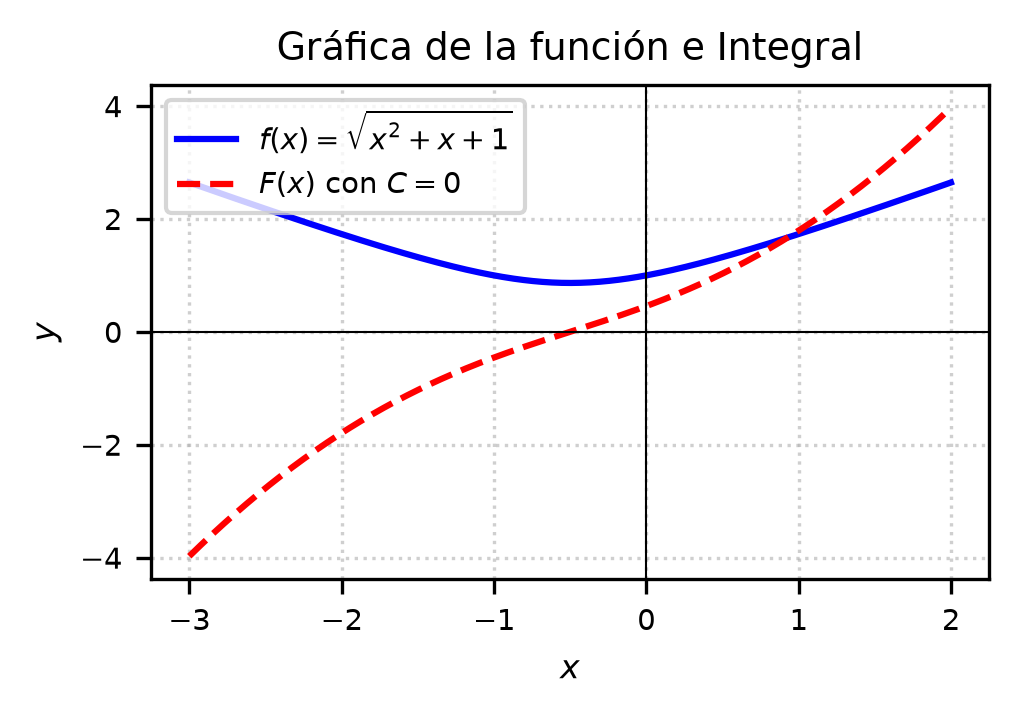
\includegraphics[width=\columnwidth]{semana_05/graficas/SEM05_P10_grafica.png}
	\caption{Representación gráfica de $f(x)$ y su antiderivada $F(x)$ evaluada para la constante de integración $C = 0$ (Problema 10).}
	\label{fig:problema10}
\end{figure}
